\subsubsection{Module MD-02: Quản lý Thực đơn \& Sản phẩm}
Module Quản lý Thực đơn \& Sản phẩm (MD-02) là một thành phần trung tâm trong hệ thống quản lý nhà hàng, đóng vai trò quan trọng trong việc định nghĩa, tổ chức và quản lý tất cả các mặt hàng mà nhà hàng cung cấp, từ món ăn, đồ uống đến các dịch vụ đi kèm. Module này cho phép Quản lý nhà hàng duy trì một cơ sở dữ liệu sản phẩm chính xác và chi tiết, làm nền tảng cho các hoạt động bán hàng, quản lý tồn kho (nếu có), và hiển thị trên giao diện Point of Sale (POS).


\begin{figure}[H]
    \centering
    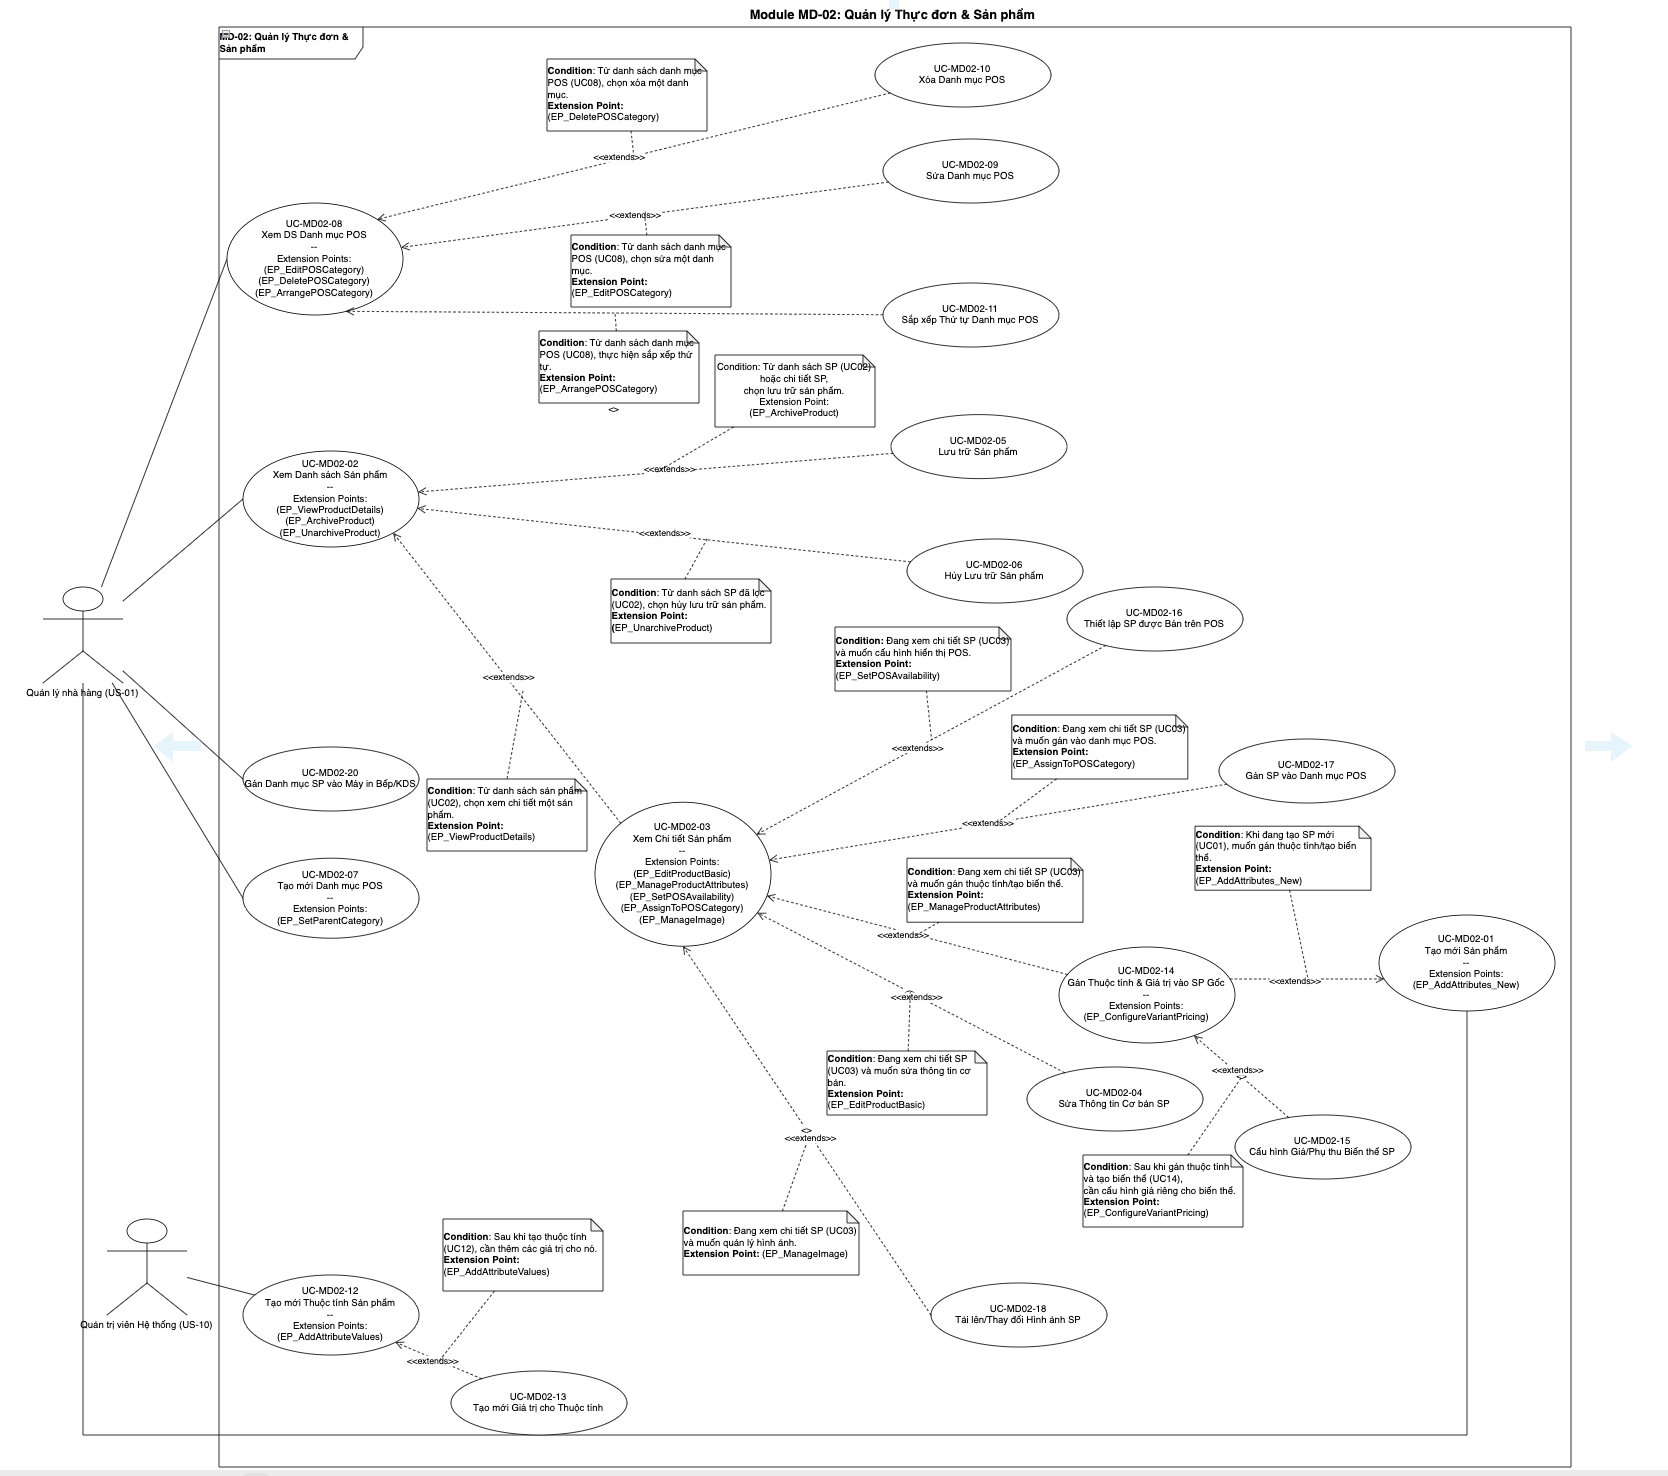
\includegraphics[width=15cm]{Sections/tong_quan/functional_spec/img/uc2.png}
    \vspace{0.5cm}
    \caption{Use case diagram cho Module MD-02}
    \label{fig:my_label}
\end{figure}

\begin{longtable}{|m{2cm}|m{2.5cm}|m{2cm}|m{4.5cm}|m{4cm}|}
\caption{Danh sách Yêu cầu Chức năng cho Module MD-02: Quản lý Thực đơn \& Sản phẩm} \label{tab:fr_md02_revised} \\
\hline
\textbf{Mã Module} & \textbf{Mã Yêu cầu CN} & \textbf{Mã Người dùng} & \textbf{Tên Chức năng} & \textbf{Mô tả Ngắn} \\
\hline
\endhead % Header cho các trang tiếp theo

\hline
\endfoot % Footer cho bảng

\hline
\endlastfoot % Footer cho trang cuối cùng

MD-02 & FR-MD02-01 & US-01 & Tạo mới Sản phẩm & Cho phép Quản lý nhà hàng thêm một món ăn, đồ uống, hoặc dịch vụ mới vào hệ thống (Tên, Giá, Loại...). \\
\hline
MD-02 & FR-MD02-02 & US-01 & Xem Danh sách Sản phẩm & Cho phép Quản lý nhà hàng xem danh sách tất cả các sản phẩm hiện có trong hệ thống. \\
\hline
MD-02 & FR-MD02-03 & US-01 & Xem Chi tiết Sản phẩm & Cho phép Quản lý nhà hàng xem thông tin chi tiết đầy đủ của một sản phẩm cụ thể. \\
\hline
MD-02 & FR-MD02-04 & US-01 & Sửa Thông tin Cơ bản của Sản phẩm & Cho phép Quản lý nhà hàng cập nhật các thông tin chung của sản phẩm (Tên, Loại, Giá bán, Giá vốn, Mã nội bộ...). \\
\hline
MD-02 & FR-MD02-05 & US-01 & Lưu trữ Sản phẩm & Cho phép Quản lý nhà hàng ẩn một sản phẩm khỏi các giao dịch mà không xóa hẳn dữ liệu (Archive). \\
\hline
MD-02 & FR-MD02-06 & US-01 & Hủy Lưu trữ Sản phẩm & Cho phép Quản lý nhà hàng kích hoạt lại một sản phẩm đã bị lưu trữ để bán/sử dụng lại (Unarchive). \\
\hline
MD-02 & FR-MD02-07 & US-01 & Tạo mới Danh mục POS & Cho phép Quản lý nhà hàng tạo một danh mục mới để nhóm sản phẩm trên giao diện POS. \\
\hline
MD-02 & FR-MD02-08 & US-01 & Xem Danh sách Danh mục POS & Cho phép Quản lý nhà hàng xem danh sách các danh mục POS đã tạo. \\
\hline
MD-02 & FR-MD02-09 & US-01 & Sửa Danh mục POS & Cho phép Quản lý nhà hàng chỉnh sửa thông tin (Tên, Thứ tự, Cha...) của một danh mục POS. \\
\hline
MD-02 & FR-MD02-10 & US-01 & Xóa Danh mục POS & Cho phép Quản lý nhà hàng xóa một danh mục POS (nếu thỏa điều kiện). \\
\hline
MD-02 & FR-MD02-11 & US-01 & Sắp xếp Thứ tự Danh mục POS & Cho phép Quản lý nhà hàng thay đổi thứ tự hiển thị của các danh mục POS. \\
\hline
MD-02 & FR-MD02-12 & US-01/US-10 & Tạo mới Thuộc tính Sản phẩm & Cho phép định nghĩa một đặc tính mới cho sản phẩm (ví dụ: Kích cỡ, Màu sắc). \\
\hline
MD-02 & FR-MD02-13 & US-01/US-10 & Tạo mới Giá trị cho Thuộc tính & Cho phép định nghĩa các lựa chọn cụ thể cho một thuộc tính (ví dụ: S, M, L cho Kích cỡ). \\
\hline
MD-02 & FR-MD02-14 & US-01 & Gán Thuộc tính và Giá trị vào Sản phẩm Gốc & Cho phép Quản lý nhà hàng áp dụng các thuộc tính và giá trị đã định nghĩa vào một sản phẩm gốc. \\
\hline
MD-02 & FR-MD02-15 & US-01 & Cấu hình Giá/Phụ thu cho Biến thể Sản phẩm & Cho phép Quản lý nhà hàng đặt giá bán khác nhau hoặc giá trị phụ thu cho từng biến thể sản phẩm cụ thể. \\
\hline
MD-02 & FR-MD02-16 & US-01 & Thiết lập Sản phẩm được Bán trên POS & Cho phép Quản lý nhà hàng đánh dấu một sản phẩm là có sẵn để bán trên POS. \\
\hline
MD-02 & FR-MD02-17 & US-01 & Gán Sản phẩm vào Danh mục POS & Cho phép Quản lý nhà hàng chỉ định một sản phẩm thuộc về (các) danh mục nào trên POS. \\
\hline
MD-02 & FR-MD02-18 & US-01 & Tải lên/Thay đổi Hình ảnh Sản phẩm & Cho phép Quản lý nhà hàng quản lý hình ảnh đại diện cho sản phẩm. \\
\hline
MD-02 & FR-MD02-19 & US-01 & Xóa Hình ảnh Sản phẩm & Cho phép Quản lý nhà hàng xóa hình ảnh hiện tại của sản phẩm. \\
\hline
MD-02 & FR-MD02-20 & US-01 & Gán Danh mục Sản phẩm vào Máy in Bếp/KDS & Cho phép Quản lý nhà hàng chỉ định danh mục sản phẩm nào sẽ gửi đến thiết bị bếp/KDS nào (Cấu hình này thường nằm trong Cài đặt POS). \\
\hline

\end{longtable}

\subsubsubsection{Mục tiêu và Phạm vi}
\label{sssec:md02_objectives_scope}
Mục tiêu chính của module MD-02 là:
\begin{itemize}
    \item \textbf{Quản lý tập trung danh mục sản phẩm:} Cung cấp một nơi duy nhất để tạo, sửa, xóa và xem thông tin chi tiết của tất cả các món ăn, đồ uống, và dịch vụ.
    \item \textbf{Hỗ trợ định giá linh hoạt:} Cho phép thiết lập giá bán, giá vốn, và quản lý giá cho các biến thể sản phẩm khác nhau.
    \item \textbf{Tổ chức thực đơn cho POS:} Cho phép tạo và quản lý các danh mục sản phẩm để hiển thị một cách khoa học và dễ sử dụng trên màn hình Point of Sale.
    \item \textbf{Quản lý biến thể sản phẩm:} Hỗ trợ tạo và quản lý các phiên bản khác nhau của cùng một sản phẩm (ví dụ: kích cỡ, độ cay, topping) với các mức giá tương ứng.
    \item \textbf{Tích hợp với các module khác:} Đảm bảo dữ liệu sản phẩm được sử dụng nhất quán trong các module Bán hàng, Kho (Inventory), Kế toán, và Point of Sale.
    \item \textbf{Cấu hình hiển thị và in ấn:} Cho phép tùy chỉnh hình ảnh sản phẩm và cấu hình cách các đơn hàng được gửi đến máy in bếp hoặc Màn hình Hiển thị Bếp (KDS).
\end{itemize}
Phạm vi của module bao gồm toàn bộ vòng đời của một sản phẩm trong hệ thống, từ việc tạo mới, cấu hình chi tiết, quản lý các thuộc tính và biến thể, tổ chức hiển thị trên POS, cho đến việc lưu trữ hoặc ngừng kinh doanh sản phẩm.

\subsubsubsection{Đối tượng Sử dụng Chính}
\label{sssec:md02_primary_users}
Module này chủ yếu được sử dụng bởi:
\begin{itemize}
    \item \textbf{US-01 (Quản lý nhà hàng):} Là người dùng chính, chịu trách nhiệm thực hiện hầu hết các chức năng của module như tạo mới sản phẩm, cập nhật giá, quản lý danh mục POS, cấu hình biến thể, và thiết lập hiển thị trên POS.
    \item \textbf{US-10 (Quản trị viên Hệ thống):} Có thể tham gia vào việc tạo và quản lý các Thuộc tính sản phẩm dùng chung hoặc các cấu hình hệ thống liên quan đến sản phẩm.
\end{itemize}
Nhân viên bán hàng (US-03) sẽ tương tác gián tiếp với module này thông qua giao diện POS, nơi họ chọn các sản phẩm đã được cấu hình.

\subsubsubsection{Các Chức năng Chính}
\label{sssec:md02_key_functionalities}
Module MD-02 cung cấp một loạt các chức năng thiết yếu, được mô tả chi tiết qua các Use Case sau:

\begin{itemize}
    \item \textbf{Quản lý Thông tin Sản phẩm Cơ bản (UC-MD02-01 đến UC-MD02-06, UC-MD02-18, UC-MD02-19):}
    \begin{itemize}
        \item Tạo mới một sản phẩm (món ăn, đồ uống, dịch vụ) với các thông tin ban đầu như tên, loại, giá bán, giá vốn (UC-MD02-01).
        \item Xem danh sách toàn bộ sản phẩm với các tùy chọn tìm kiếm, lọc và nhóm (UC-MD02-02).
        \item Xem thông tin chi tiết đầy đủ của một sản phẩm cụ thể (UC-MD02-03).
        \item Sửa đổi các thông tin cơ bản của sản phẩm đã tồn tại (UC-MD02-04).
        \item Lưu trữ (ẩn đi) các sản phẩm không còn kinh doanh và hủy lưu trữ khi cần (UC-MD02-05, UC-MD02-06).
        \item Tải lên, thay đổi hoặc xóa hình ảnh đại diện cho sản phẩm (UC-MD02-18, UC-MD02-19).
    \end{itemize}

    \item \textbf{Quản lý Danh mục Point of Sale (POS) (UC-MD02-07 đến UC-MD02-11):}
    \begin{itemize}
        \item Tạo mới các danh mục để phân loại sản phẩm trên giao diện POS (ví dụ: "Khai vị", "Món chính") (UC-MD02-07).
        \item Xem, sửa, xóa và sắp xếp thứ tự hiển thị của các danh mục POS (UC-MD02-08, UC-MD02-09, UC-MD02-10, UC-MD02-11).
    \end{itemize}

    \item \textbf{Quản lý Thuộc tính và Biến thể Sản phẩm (UC-MD02-12 đến UC-MD02-15):}
    \begin{itemize}
        \item Tạo mới các thuộc tính chung cho sản phẩm (ví dụ: "Kích cỡ", "Màu sắc", "Độ cay") (UC-MD02-12).
        \item Định nghĩa các giá trị cụ thể cho từng thuộc tính (ví dụ: "Nhỏ", "Vừa", "Lớn" cho thuộc tính "Kích cỡ") (UC-MD02-13).
        \item Gán các thuộc tính và giá trị đã chọn vào một sản phẩm gốc, từ đó tự động tạo ra các sản phẩm biến thể (UC-MD02-14).
        \item Cấu hình giá bán riêng hoặc mức phụ thu cho từng biến thể sản phẩm cụ thể (UC-MD02-15).
    \end{itemize}

    \item \textbf{Cấu hình Sản phẩm cho Point of Sale (UC-MD02-16, UC-MD02-17, UC-MD02-20):}
    \begin{itemize}
        \item Thiết lập cho phép hoặc không cho phép một sản phẩm được bán trên giao diện POS (UC-MD02-16).
        \item Gán một sản phẩm vào một hoặc nhiều danh mục POS để hiển thị đúng nhóm trên menu (UC-MD02-17).
        \item Cấu hình việc định tuyến các danh mục sản phẩm đến các máy in bếp hoặc màn hình KDS cụ thể khi có đơn hàng (UC-MD02-20).
    \end{itemize}
\end{itemize}

\subsubsubsection{Tóm tắt Luồng Hoạt động Tổng thể}
\label{sssec:md02_overall_workflow}
Luồng hoạt động điển hình trong module Quản lý Thực đơn \& Sản phẩm bao gồm các bước chính sau:
\begin{enumerate}
    \item \textbf{Tạo sản phẩm mới:} Quản lý nhà hàng Tạo mới Sản phẩm với các thông tin cơ bản như tên, giá, loại (UC-MD02-01).
    \item \textbf{Cấu hình chi tiết sản phẩm:}
        \begin{itemize}
            \item Tải lên Hình ảnh Sản phẩm (UC-MD02-18).
            \item Nếu sản phẩm có nhiều phiên bản, Quản lý sẽ Tạo mới Thuộc tính (UC-MD02-12), Tạo mới Giá trị cho Thuộc tính (UC-MD02-13), Gán Thuộc tính và Giá trị vào Sản phẩm Gốc để tạo biến thể (UC-MD02-14), và Cấu hình Giá/Phụ thu cho Biến thể (UC-MD02-15).
        \end{itemize}
    \item \textbf{Chuẩn bị cho POS:}
        \begin{itemize}
            \item Quản lý Tạo mới Danh mục POS nếu cần (UC-MD02-07) hoặc Sắp xếp Thứ tự Danh mục POS (UC-MD02-11).
            \item Thiết lập Sản phẩm được Bán trên POS (UC-MD02-16).
            \item Gán Sản phẩm vào Danh mục POS tương ứng (UC-MD02-17).
            \item Gán Danh mục Sản phẩm vào Máy in Bếp/KDS để định tuyến đơn hàng (UC-MD02-20).
        \end{itemize}
    \item \textbf{Bảo trì và cập nhật:}
        \begin{itemize}
            \item Quản lý thường xuyên Xem Danh sách Sản phẩm (UC-MD02-02) và Xem Chi tiết Sản phẩm (UC-MD02-03).
            \item Thực hiện Sửa Thông tin Cơ bản của Sản phẩm khi cần (ví dụ: thay đổi giá) (UC-MD02-04).
            \item Lưu trữ Sản phẩm không còn kinh doanh (UC-MD02-05) hoặc Hủy Lưu trữ Sản phẩm khi muốn bán lại (UC-MD02-06).
            \item Quản lý Danh mục POS: Sửa (UC-MD02-09) hoặc Xóa (UC-MD02-10) khi cần thiết.
        \end{itemize}
\end{enumerate}
Module MD-02 đảm bảo rằng thực đơn của nhà hàng luôn được cập nhật, chính xác và được trình bày một cách tối ưu trên các hệ thống bán hàng, góp phần vào trải nghiệm khách hàng tốt và hiệu quả vận hành.
